\documentclass[proof]{beamer}
\usetheme{default}

\usecolortheme{rose}
\usepackage[english]{babel}
\usepackage[utf8]{inputenc}
%\usepackage[latin1]{inputenc}
 \usepackage{amssymb}
 \usepackage{latexsym}
 \usepackage{amsmath}
 \usepackage{amssymb}
 \usepackage{tikz}
 \usepackage{tikz-cd}
\usepackage{array}
\usepackage{rotating}
\usepackage{forest}
\usepackage{color}
\usepackage[all,cmtip]{xy}
\usepackage{stmaryrd}

\usepackage{pgfplots}
\usepackage{array}
    \newcolumntype{C}{>{\centering\arraybackslash}c}



\definecolor{qbblue}{RGB}{43,126,128}
%\definecolor{qbblue}{RGB}{43,126,204}
\definecolor{qborange}{RGB}{242,151,36}
\definecolor{qblight}{RGB}{210,210,210}
\definecolor{qbdark}{RGB}{180,180,180}
\definecolor{qbred}{RGB}{184,13,72}

\setbeamercolor{title}{fg=black}
\setbeamercolor{section in toc}{fg=black}
\setbeamercolor{block title}{bg=qblight,fg=black}
\setbeamercolor{frametitle}{bg=qblight,fg=black}
\setbeamercolor{section in head/foot}{bg=black}
\setbeamertemplate{itemize item}{\color{qbdark}$\blacktriangleright$}
\setbeamertemplate{itemize subitem}{\color{qbdark}$\blacktriangleright$}
%\setbeamercolor*{palette tertiary}{bg=black}
\setbeamercolor{local structure}{fg=black}

\usepackage[style=verbose,backend=biber]{biblatex}
\addbibresource{biblio.bib}

\renewcommand{\_}{\rule{.6em}{.5pt}\hspace{0.023cm}}

\newcommand{\bloc}[2]{\begin{block}{#1}\setlength\abovedisplayskip{0pt}#2\end{block}}

\setbeamertemplate{navigation symbols}{} 
\addtobeamertemplate{footline}{\hfill{\tiny \insertframenumber}\hspace{2em} \vspace{1em}}

\newcommand{\red}[1]{\textcolor{qbred}{#1}}
\newcommand{\blue}[1]{\textcolor{qbblue}{#1}}
\newcommand{\orange}[1]{\textcolor{qborange}{#1}}

\newcommand{\D}{\mathbb{D}}
\newcommand{\bP}{\mathbb{P}}
\newcommand{\propTrunc}[1]{\lVert #1 \rVert}
\newcommand{\eqspace}{\vspace{0.32cm}}

\newcommand{\SB}{\text{SB}}
\newcommand{\AZ}{\text{AZ}}
\newcommand{\LI}{\Phi}
\newcommand{\B}{\text{B}}
\newcommand{\Et}{\text{\'Et}}
\newcommand{\Aut}{\text{Aut}}
\newcommand{\PGL}{\text{PGL}}
\newcommand{\U}{\text{U}}
\newcommand{\Spec}{\text{Spec}}
\renewcommand{\lim}{\text{lim}}
\newcommand{\M}{\text{M}}

\def\mhyphen{{\hbox{-}}}

\newcommand{\Alg}{\text{Alg}}
\newcommand{\T}{\mathbb{T}}
\newcommand{\G}{\mathbb{G}}
\newcommand{\Hom}{\text{Hom}}
\newcommand{\Set}{\text{Set}}
\newcommand{\N}{\mathbb{N}}
\newcommand{\DM}{\text{DM}}

%\newcommand{\trunc}[1]{|| #1 ||}

\AtBeginSection[]
{
 \begin{frame}<beamer>
 \frametitle{Outline}
 \tableofcontents[currentsection]
 \end{frame}
}

\begin{document}


%\abovedisplayskip=0.0cm
%\abovedisplayshortskip=-0.3cm
%\belowdisplayskip=0.6cm


\title{\red{In Memory of Tim Lichtnau:\\
Deligne-Mumford Stacks in Synthetic Algebraic Geometry}}
\author{Felix Cherubini and Hugo Moeneclaey,\\
\vspace{0.16cm}
after Tim Lichtnau's master thesis notes\\
}
\date{\blue{HoTT/UF 2026}\\
Aarhus}



\frame{\titlepage}




\frame{\frametitle{Tim Lichtnau}

Tim died on the 26th of December 2024.
\vspace{0.2cm}
\begin{figure}
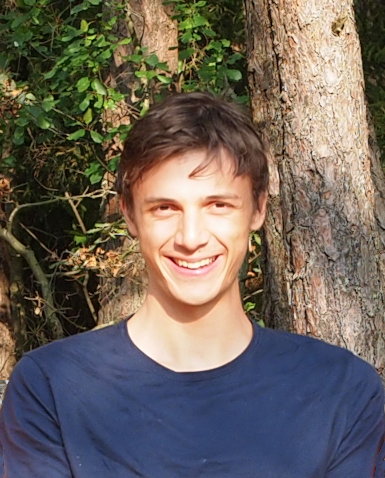
\includegraphics[width=0.4\textwidth]{images/tim.png}
\end{figure}

In this talk I will present work from his unfinished master thesis.

}


\frame{\frametitle{Overview}

Tim's master thesis was about Deligne-Mumford stacks in synthetic algebraic geometry.

\bloc{Intuition}{
Deligne-Mumford stacks are $1$-types which are ``nice'' quotients of schemes.
}

Tim gave an extension to $n$-types, based on [Simpson 96].

\begin{center}
``In this paper we simply \emph{assume} that a theory of $n$-stacks\footnote{aka sheaves of $n$-groupoids} of groupoids exists.''
\end{center}

\bloc{HoTT gives such a theory!}{
\begin{itemize} 
\item The $n$-groupoid structure can be modelled using $n$-types.
\item Sheafification is an accessible lex modality.
\end{itemize}
}

}


% \begin{frame}<beamer>
% \frametitle{Outline}
% \tableofcontents
% \end{frame}
 

\section{From affine schemes to Deligne-Mumford stacks}


%\frame{\frametitle{Affine schemes}

%We want to study roots of system of polynomials over an arbitrary ring.

%\bloc{Key idea}{
%Given a polynomial $P$, we construct a space of its roots, called an affine scheme.
%}

%\bloc{Traditional approach (over a given base ring $k$)}{
%Define it as the Zariski sheaf sending a $k$-algebra $A$ to $\{x:A\ |\ P(x)=0\}$.

%This embeds $k$-algebras in Zariski sheaves.
%}

%\bloc{Synthetic approach (over the generic ring $R$)}{
%Define it as the set $\{x:R\ |\ P(x)=0\}$.

%This embeds finitely presented $R$-algebras in sets.
%}

%}

\frame{\frametitle{Affine schemes}

%\bloc{Reminder}{
%An affine scheme is a type merely of the form:
%\[\{x_1,\hdots,x_n:R\ |\ P_1(x)=0, \hdots, P_m(x)=0\}\]
%for some $P_1,\hdots,P_m:R[X_1,\hdots,X_n]$.
%}

%\bloc{Reminder}{
%An affine schemes are defined as the set of roots of some system of polynomials
%}

\bloc{Duality axiom}{
We have an equivalence

\[R\mhyphen \Alg_{\mathrm{f.p.}}  \simeq \{\text{Affine\ schemes}\}.\]

%\begin{center}
%\begin{tabular}{ccc}
%$R\mhyphen \Alg_{f.p.}$ & $\simeq$ & $\{\text{Affine\ schemes}\}$. \\
%$A$ & $\mapsto$ &  $\Hom_{R\mhyphen\Alg}(A,R)$\\
%$R^X$ & $\mapsfrom$ & $X$
%\end{tabular}
%\end{center}
}

For affine schemes, algebra and geometry match up perfectly.

}


%\frame{\frametitle{Schemes}

%\bloc{Definition (Traditional)}{
%A scheme is a Zariski sheaf that has an open cover by affine pieces.
%}

%\bloc{Definition (Synthetic)}{
%A scheme is a set that has a finite open cover by affine pieces.
%}

%\bloc{Example}{
%Given $n:\mathbb{N}$, the type $\bP^n = \{Lines in R^{n+1} going through 0\}$ is a scheme.
%}

%Core idea: locally we can use algebra

%}


\frame{\frametitle{But not everything is affine}

Assume $n>0$.

\bloc{Definition}{
We define the projective space $\bP^n$ by

\[\bP^n = \{\text{Lines\ in}\ R^{n+1}\ \text{going\ through}\ 0\}.\]
}

Any map in from $\bP^n$ to $R$ is constant, so $\bP^n$ cannot be affine.

\bloc{Definition}{
A scheme is a set that has a finite open cover by affine pieces.
}

\bloc{Example}{
$\bP^n$ is a scheme.
}

}


\frame{\frametitle{But not everything is a scheme}

\bloc{Definition}{
A cubic surface is a scheme $X$ such that there exists $P:R[X_0,\cdots,X_3]$ homogeneous of degree $3$ with 

\[X = \{x:\bP^3\ |\ P(x)=0\}.\]
}

\bloc{Remark}{
The type of smooth cubic surfaces is nice:
\begin{itemize}
\item We have a surjection $\bP^{19}\to \{\text{Cubic\ surfaces}\}$.
\item Being smooth is an open condition.
\end{itemize}
}

But it cannot be a scheme, it is not even a set!

}


\frame{\frametitle{Smooth cubic surfaces and the 27 lines}

\bloc{Theorem (over $k$ an algebraically closed field)}{
Any smooth cubic surface contains precisely 27 lines.
}

\begin{figure}
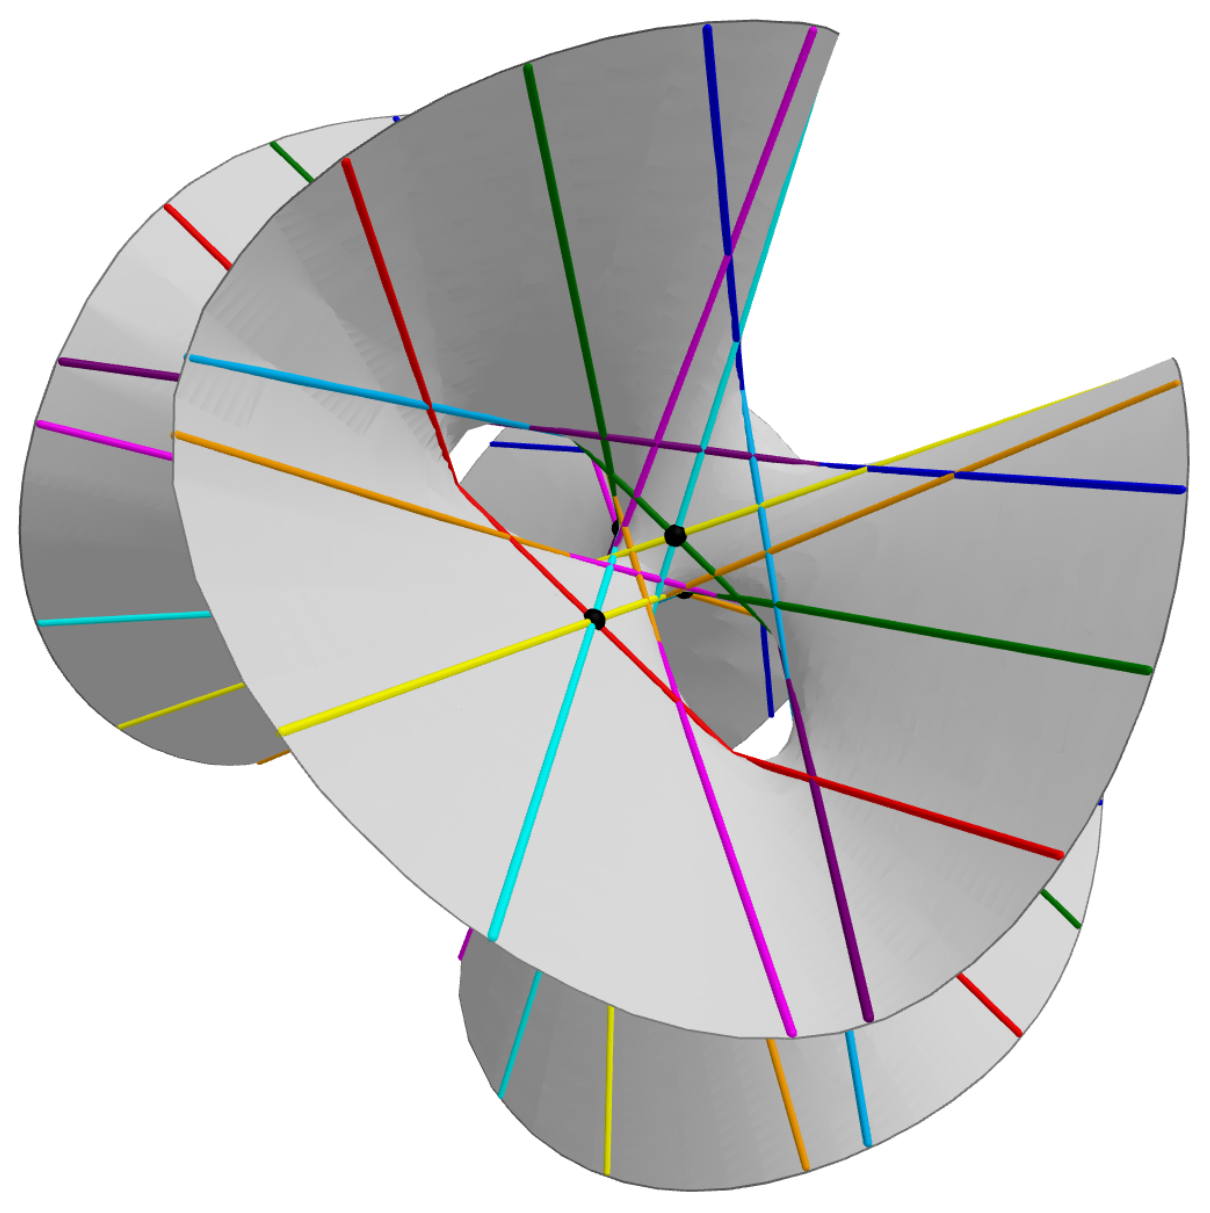
\includegraphics[width=0.4\textwidth]{images/cubic_surface.png}
\end{figure}

This gives a tight control on automorphisms of these surfaces.

}


\frame{\frametitle{Deligne-Mumford stacks}

The notion of DM stack captures this intuition. 

\bloc{Intuition}{
A Deligne-Mumford stack is a $1$-type that is:
\begin{itemize} 
\item An étale sheaf.
\item \'Etale-locally affine.
\end{itemize}
}

\bloc{Why \'etale-locally?}{
A type that is Zariski-locally affine is a set.
}

\bloc{Higher Deligne-Mumford stacks [Simpson 96]}{
Moduli spaces of Deligne-Mumford stacks are usually $2$-types, etc...
}

}


%\frame{\frametitle{Why do it synthetically?}

%\bloc{Traditional approach}{
%A Deligne-Mumford $n$-stack is a presheaf of $n$-groupoids on the \'etale site such that:
%\begin{itemize}
%\item It is a stack (i.e.\ a sheaf of $n$-groupoids).
%\item It is \'etale locally affine.
%\end{itemize}
%}

%\bloc{Synthetic approach}{
%A Deligne-Mumford $n$-stack is an $n$-type such that:
%\begin{itemize}
%\item It is an \'etale sheaf (i.e.\ it is modal, same as for sets).
%\item It is \'etale locally affine.
%\end{itemize}
%}

%}


\frame{\frametitle{What to expect synthetically?}

\bloc{Traditional approach}{
Use sheaves of $n$-groupoids (aka $n$-stack) on the \'etale site.
}

<<<<<<< HEAD
$\Rightarrow$ A lot of technical machinery needed.
=======
$\Rightarrow$ A lot of technical machinery is needed.
>>>>>>> 70288afb7d12974ec1b352ef784f1588100ffe41

\bloc{Synthetic approach}{
\begin{itemize}
\item Sheaves of $n$-groupoids on the Zariski site are just $n$-types. 
\item \'Etale sheaves are modal types for some accessible lex modality.
\end{itemize}
}

$\Rightarrow$ We expect a more direct and elegant development.

}



\section{Synthetic Deligne-Mumford stacks}

\frame{\frametitle{Formally \'etale types}

\bloc{Definition}{
A type $X$ is formally \'etale if given any $\epsilon:R$ nilpotent, the map:

\[X\to X^{\epsilon=0}\]
is an equivalence.
}

\bloc{Intuition}{
\begin{itemize}
\item $\epsilon$ nilpotent means $\epsilon$ infinitesimal.
%\item $X$ formally \'etale means $X$ thinks infinitesimal are $0$.
%\item $X$ formally \'etale means infinitesimal don't matter when working in $X$
\item $X$ formally \'etale means $X$ discrete.
\end{itemize}
}

}


\frame{\frametitle{\'Etale sheaves}

\bloc{Definition}{
An \'etale cover is a map whose fibers are formally \'etale and non-empty.
}

\bloc{Definition}{
A type $X$ is an \'etale sheaf if for all $S$ affine, formally \'etale and non-empty, we have that

\[X\to X^{\propTrunc{S}}\]
is an equivalence.
}

\bloc{Intuition}{
\begin{itemize}
\item \'Etale sheaves ``see'' affine \'etale covers as surjections.
\item If we have a goal which is an  \'etale sheaf, we can assume e.g.\ that separable polynomials have roots. 
\end{itemize}
}

}


\frame{\frametitle{Deligne-Mumford stacks}

%\bloc{Definition}{
%We define the class $CS$ of covering stacks the smallest $CS\subset etale sheaves$ such that:
%\begin{itemize}
%\item $\mathbb{T}\subset CS$.
%\item If $S:\mathbb{T}$ and $p:S\to X$ whose fibers are in $CS$, then $X\in CS$.
%\end{itemize}
%}

Now we define the class of Deligne-Mumford stacks.

\bloc{Definition}{
$\DM$ is the smallest class of \'etale sheaves such that:
\begin{itemize}
\item $S$ affine $\Rightarrow S\in\DM$.
\item $S$ affine, $p:S\to X$ \'etale cover with fibers in $\DM$\ \ $\Rightarrow X\in\DM$.
\end{itemize}
}

%\bloc{Definition}{
%A Deligne-Mumford stack is an étale sheaf $X$ such that there exists $S$ affine and $p:S\to X$ whose fibers are in CS.
%}

%\bloc{Intuition}{
%Given $X$ a Deligne-Mumford stack,
%\[X\in CS iff X formally and not not X\]
%}

}


\frame{\frametitle{Stability properties for Deligne-Mumford stacks}

\bloc{Proposition}{
\begin{itemize}
\item $\DM$ is stable under $\Sigma$ and identity types.
%\item $(X\in \DM,Y:X\to\DM) \Rightarrow \Sigma_XY\in\DM$
%\item $(X\in\DM, x,y:X) \Rightarrow x=_Xy\in \DM$.
\item Given $Y$ an \'etale sheaf with $X\in \DM$ and $p:X\to Y$ an \'etale cover with fibers in $\DM$, we have that $Y\in \DM$.
\end{itemize}
}

\bloc{Proposition}{
The type of Deligne-Mumford stacks is an \'etale sheaf.
}

Traditionally called \'etale descent for Deligne-Mumford stacks.

}


\section{Algebraic spaces that are not schemes}


\frame{\frametitle{Algebraic spaces}

\bloc{Definition}{
An algebraic space is a Deligne-Mumford stack which is a set\footnote{Traditionally, identity types in algebraic spaces are required to be schemes.}.
}

%\bloc{Warning!}{
%Traditionally we would require its identity types to be schemes.
%}

\bloc{Intuition}{
\begin{itemize}
\item A scheme is a set that is Zariski-locally affine.
\item An algebraic space is a set that is \'etale-locally affine.
\end{itemize}
}

We want interesting examples of those.

}


\frame{\frametitle{Algebraic spaces that are not schemes}

Tim proved the following chain of strict inclusions.

\begin{center}
\begin{tabular}{ccccc}
$\{\text{Schemes}\}$ & $\subsetneq$ & 
$\left\{\begin{tabular}{c}
$\text{Locally\ separated}$ \\
$\text{algebraic\ spaces}$ 
\end{tabular} \right\}$&
$\subsetneq$ & $\left\{\text{Algebraic\ spaces}\right\}$\\
\end{tabular}
\end{center}

}


%\frame{\frametitle{A non-locally separated algebraic space}

%Assume $2$ an invertible prime, $\mu_l = \{x:R\ |\ x^l=1\}$ acts on $R$.

%\bloc{Lemma}{
%For $x,y:R$, define:
%\[(x\sim y) = (x=y)\lor (x\not=0)\land (y\not=0)\land \exists(g:\mu^l) gx=y\]
%}

%\bloc{Lemma}{
%$R/\sim$ is an algebraic space that is not locally separated.
%}

%}


\frame{\frametitle{A non-locally separated algebraic space}

Assume $2$ invertible in $R$.

\bloc{Lemma}{
For $x,y:R$, define:

\[(x\sim y) = (x=y)\lor (x\not=0)\land (y\not=0)\land (x=-y)\]
}

\bloc{Lemma}{
$R/\sim$ is an algebraic space that is not locally separated.
}

}


\frame{\frametitle{A locally separated algebraic space that is not a scheme}

Assume $2$ invertible in $R$.

\bloc{Definition}{
Given $r:R^\times$, we define:

\[D_r = \{x:R,\, y:R/x\ |\ y^2 = r\ \text{mod}\ x\}\]
}

\bloc{Intuition}{
\begin{itemize}
\item $D_1$ is the line with two origins.
\item $D_r$ is the line with the square roots of $r$ as origins.
\end{itemize}
}

\bloc{Lemma}{
Consider $H=\Sigma_{r:R^\times} D_r$, then:
\begin{itemize}
\item $H$ is a locally separated algebraic space.
\item $H$ is not a scheme.
\end{itemize}
}

%Is there a separated algebraic space that is not a scheme?

}


\frame{\frametitle{Where next?}

...

}


\end{document}
